% Chapter Template

\chapter{Dataset} % Main chapter title

\label{ch:04} % Change X to a consecutive number; for referencing this chapter elsewhere, use \ref{ChapterX}

%----------------------------------------------------------------------------------------
%	SECTION 1
%----------------------------------------------------------------------------------------

In this work, we need two types of input data to train our models. 
First, we need to know the geometry of the object surface. This can be captured by a depth camera, which records the distance of the object surface from the optical center of the camera and can be converted into a point cloud. 
Second, we need information about the illumination of the object surface, which is used as photometric information for further improvements. 
This type of information requires an observed image of the object with the light directions projected onto the object surface. 

To obtain this data, we can use a structured light scanner to scan the objects in the laboratory. However, the scanner usually cannot scan the dark, shiny, and transparent areas, resulting in many missing pixels and holes in the depth map. This incomplete surface information makes it difficult to train our model because the ground truth corresponding to the depth map is also incomplete. Second, training a deep learning-based model usually requires a large dataset, especially for a network without a backbone. Creating a single deep map dataset for this work would require too much work and resources. A suitable way to obtain huge depth map data with illumination information is to use a game engine that can simulate an arbitrary number of data.

We use the Unity game engine for data generation. Using a $ C\# $ script, we can set up a similar configuration in the lab. We then create a dataset based on the collected objects. The dataset we created for this work is called \textit{synthetic-50-5} because it contains 50 different object models for training and 5 object models for testing.

\section{Data Resources}
The object models we used were collected from the Internet.
A number of point cloud datasets for image processing research have been published by \cite{data1}, \cite{data2}, \cite{data3}, and \cite{data4}. Some of these point clouds were scanned from real objects using high-resolution scanners such as the Cyberware 3030 MS+ and calibrated with post-processing. These objects were scanned hundreds of times, fully capturing the original objects with up to millions of points\cite{data1}. Some of them are fully digitally synthesized. The dense point clouds make the normal inference task trivial, as the neighborhood-based method works adequately for this type of task. Some of the point clouds even contain precomputed normal maps based on more advanced methods. They all provide the accurate ground truth for the supervised learning method.

The \textit{synthetic-50-5} is a dataset we created in this work based on 50 point clouds as the training set and 5 point clouds as the test set. In creating the dataset, we tried to use as many object types as possible to cover a robust and wide range of training scenarios. There are several categories of models, such as figurines, animals, statues, toys, furniture, antiques, and car models, some of which have relatively smooth surfaces, such as model \textit{arm, bus, rabbit, cat, zebra}, and some of which have very intricate details, such as model \textit{Washington, Car-Engine, Armadillo}. 
We created this dataset for normal inference tasks. Figure \ref{fig:dataset-demo} shows illustrations of some objects. Appendix \ref{AppendixA} contains a complete version of the models of the dataset.


\begin{figure}[!h]
	\centering
	\captionsetup{width=\linewidth}
	\begin{subfigure}[b]{0.24\linewidth}
		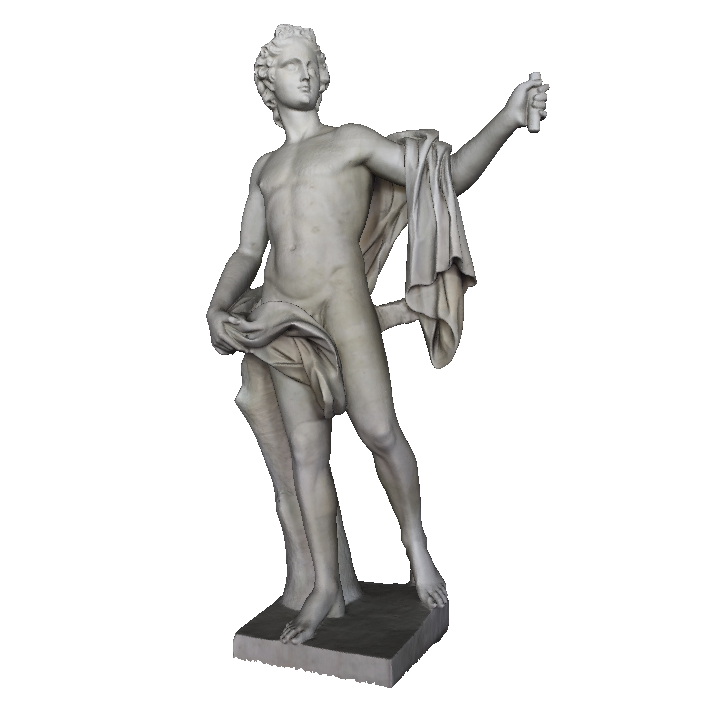
\includegraphics[width=\linewidth]{./Figures/train-dataset/00.apoll.png}
		\caption{apoll}
	\end{subfigure}
	\begin{subfigure}[b]{0.24\linewidth}
		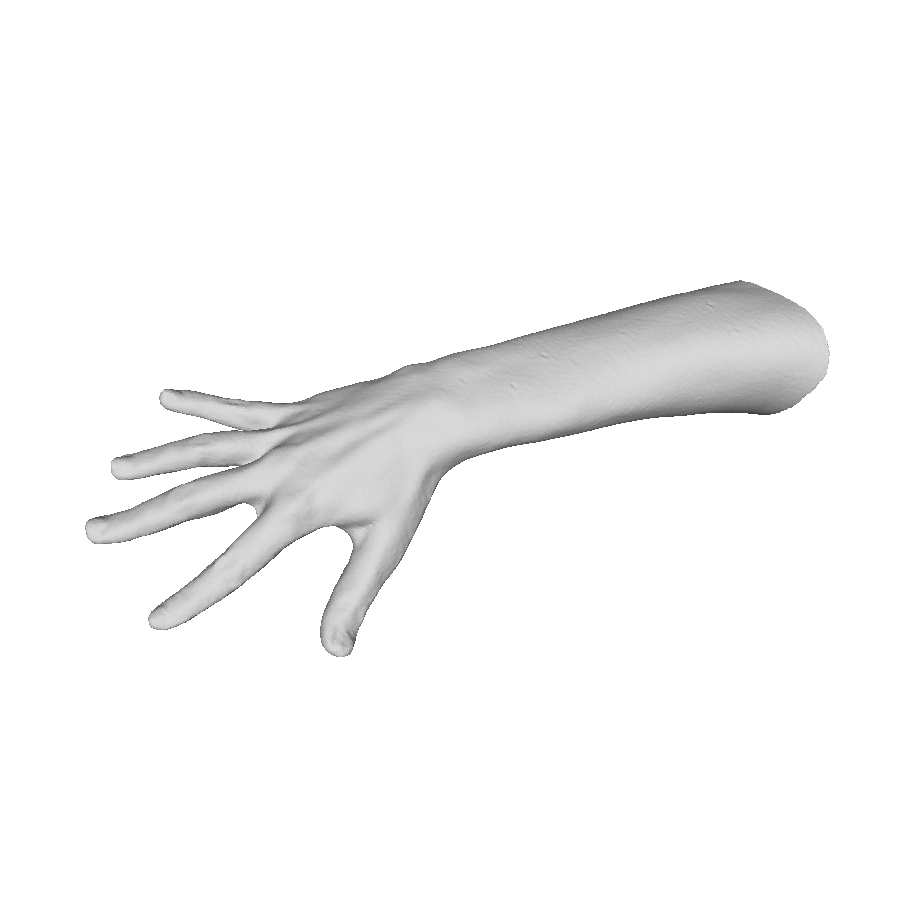
\includegraphics[width=\linewidth]{./Figures/train-dataset/01.arm.png}
		\caption{arm}
	\end{subfigure}
	\begin{subfigure}[b]{0.24\linewidth}
		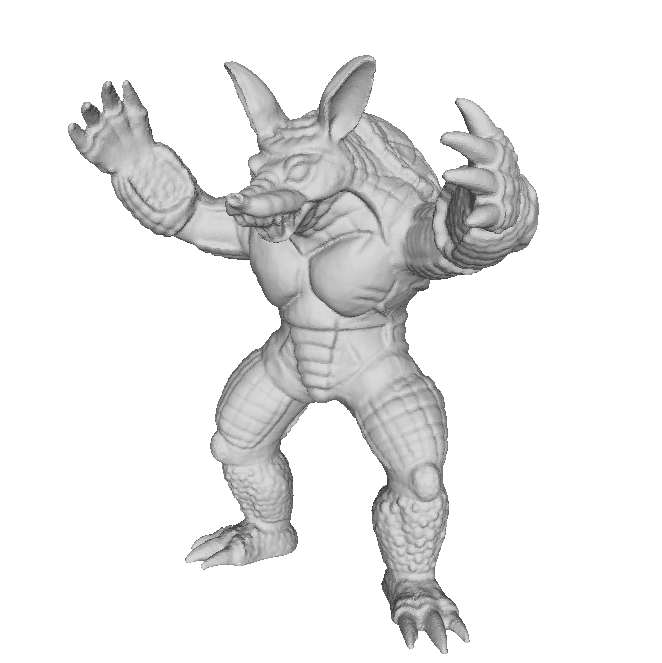
\includegraphics[width=\linewidth]{./Figures/train-dataset/02.armadillo.png}
		\caption{armadillo}
	\end{subfigure}
	\begin{subfigure}[b]{0.24\linewidth}
		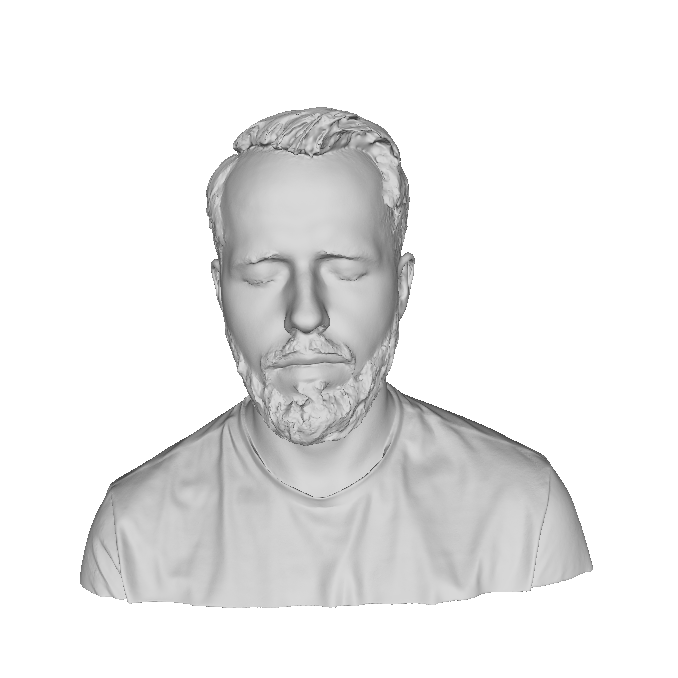
\includegraphics[width=\linewidth]{./Figures/train-dataset/03.bearded-guy.png}
		\caption{bearded-guy}
	\end{subfigure}
	
	\begin{subfigure}[b]{0.24\linewidth}
		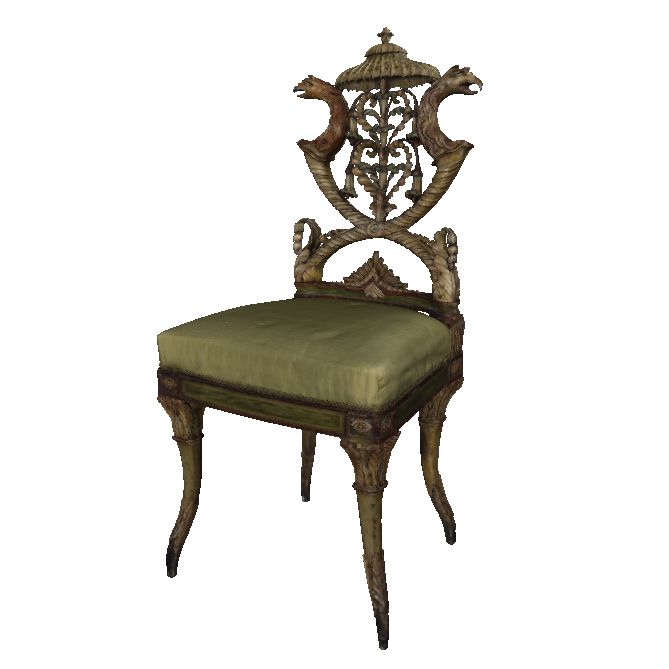
\includegraphics[width=\linewidth]{./Figures/train-dataset/08.pergolesi-side-chair_texture.png}
		\caption{chair}
	\end{subfigure}
	\begin{subfigure}[b]{0.24\linewidth}
		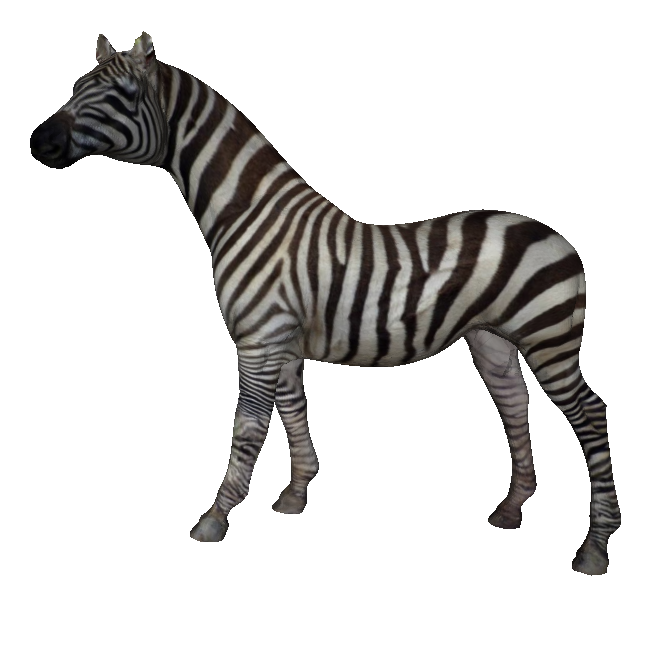
\includegraphics[width=\linewidth]{./Figures/train-dataset/42.zebra_texture.png}
		\caption{zebra}
	\end{subfigure}
	\begin{subfigure}[b]{0.24\linewidth}
		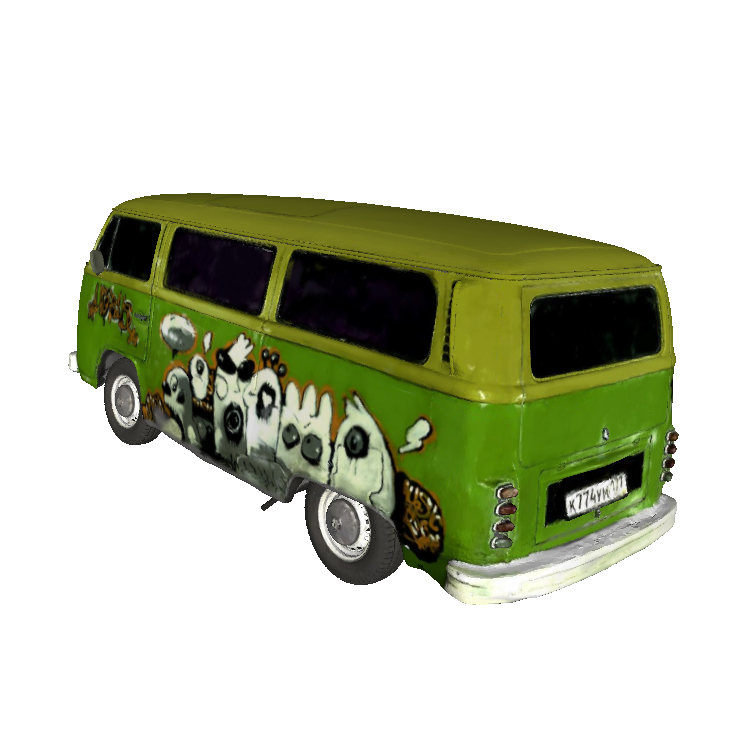
\includegraphics[width=\linewidth]{./Figures/test-dataset/01.bus_texture.png}
		\caption{bus}
	\end{subfigure}
	\begin{subfigure}[b]{0.24\linewidth}
		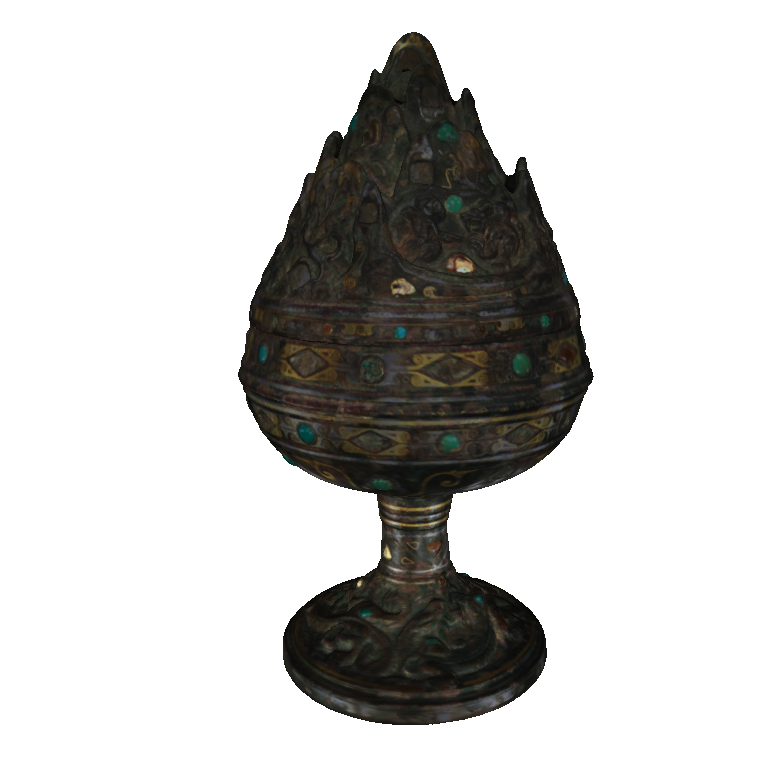
\includegraphics[width=\linewidth]{./Figures/test-dataset/03.baoshanlu_texture.png}
		\caption{baoshanlu}
	\end{subfigure}
	\decoRule
	\caption{Some of the objects used for \textit{Synthetic-50-5}}
	\label{fig:dataset-demo}
\end{figure}
In addition, some objects also have colored textures, as shown in the second line of Figure \ref{fig:dataset-demo}. This is specifically prepared for the illuminated approach, since the image is used to evaluate the surface normals. By using textured models, our models get closer to the real dataset and have improved robustness that can be further applied to the real dataset.



\definecolor{direction-light-color}{RGB}{255,244,214}
\newcommand{\col}[1]{%
	\textcolor{#1}{\vrule width 0.5cm}}
\section{Synthesizing Scenes using Unity}

To simulate the data acquisition scenario as realistically as possible. We made the following settings. A flat cylinder, called \textit{stage} , is placed in the center of the 3D space as a platform for placing objects. We fixed the \textit{stage} in a predetermined position that will not be changed when images are captured. 
A directional light with RGB color FFF4D6 \col{direction-light-color} is placed 25 m away in the top view direction as an ambient light, which also has a fixed position.
An RGB-D camera is placed about 10 m away from the stage in the top-view direction. The camera captures the depth map and the grayscale image, which are randomly arranged after each scene. The movement range of the camera is 0.1 m in both directions of the X, Y and Z axes and a randomly changed Euler angle of $ 1^\circ $. 
A point light is placed about 5 m away as the illumination light, which is also moved randomly after each scene. The range of motion is 0.3 m in both directions of the X, Y and Z axes and $ 1^\circ $ randomly in the Euler angle.

During data acquisition, the object is randomly selected and placed on the stage. The object has a random rotation of up to $ 30^\circ $ in the $roll $ axis direction, a $ 30^\circ $ rotation in the $pitch $ axis direction, and a $ 180^\circ $ degree rotation in the $yaw $ axis direction. This gives the camera the ability to capture most directions of the objects. The layout in the Unity game engine is shown in Figure \ref{fig:unity-workplace}. We generate 3000 scenes with resolution $ 128\times128 $ and 5000 scenes with resolution $ 512\times512 $.

\begin{figure}[h!]
	\centering
		\captionsetup{width=\linewidth}
	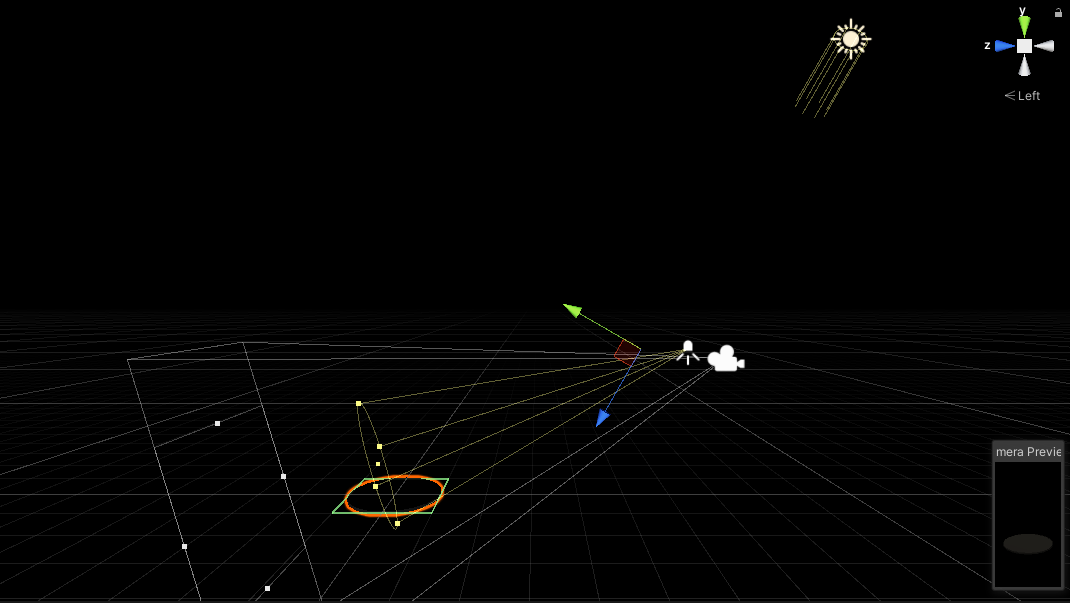
\includegraphics[width=\linewidth]{./Figures/unity-workplace.PNG}
	\decoRule
	\caption{The layout of synthetic scene generation in Unity.}
	\label{fig:unity-workplace}
\end{figure}
The main advantage of generated scenes is the availability of complete information. We can capture the depth map in a lossless way. The corresponding normal map can also be safely considered as ground truth. And the scale of the dataset is easy to control. Table \ref{tab:data-files} gives more dataset information.
\begin{table}
	\centering
	\begin{tabular}{l l}
		\toprule
		\tabhead{Data} & \tabhead{Size} \\
		\midrule
		Depth map & Width$ \times $Height$ \times $ 1 \\
		\hline 
		Depth range  & MinDepth, MaxDepth \\  
		\hline
		Grayscale Image	&  Width$ \times $Height$ \times $ 1 \\  
		\hline 
		Normal Map &   Width$ \times $Height$ \times $ 3  \\
		\hline 
		Light Position &  $ 3\times1 $  \\
		\hline
		Camera Intrinsic Matrix &  $ 3\times 3 $  \\
		\hline 
		Camera Extrinsic Matrix &  $ 3\times 4 $  \\
		\hline 
		\bottomrule
	\end{tabular}
	\caption{The information saved for each scene in \textit{synthetic-50-5}.}
	\label{tab:data-files}
\end{table}


A critical detail we need to pay attention to is the exposure of the camera. Or we need to control the light emission on the object surface. As can be seen in Figure \ref{fig:camera_exposure}, too much exposure causes the surface texture to be difficult to see, resulting in clipping. In our experiments, we found that an appropriate light setting is essential for the illumination-based approach. Too much or too little lighting effects do not improve the illumination-based approach.

\begin{figure}[H]
	\centering
	\captionsetup{width=\linewidth}
	\begin{subfigure}[b]{0.32\linewidth}
		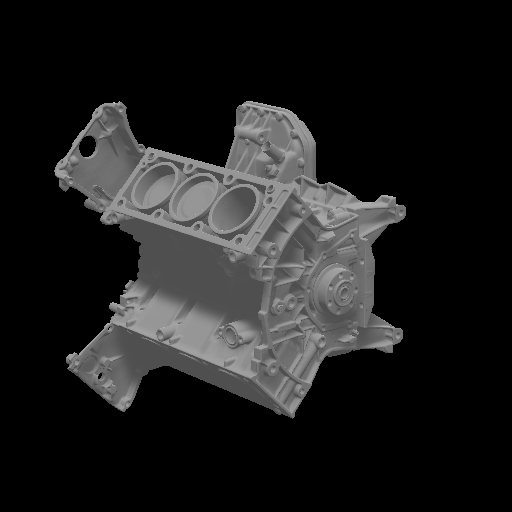
\includegraphics[width=\textwidth]{./Figures/wrong_exposure_2.png}
		\caption{Insufficient light}
	\end{subfigure}
	\begin{subfigure}[b]{0.32\linewidth}
		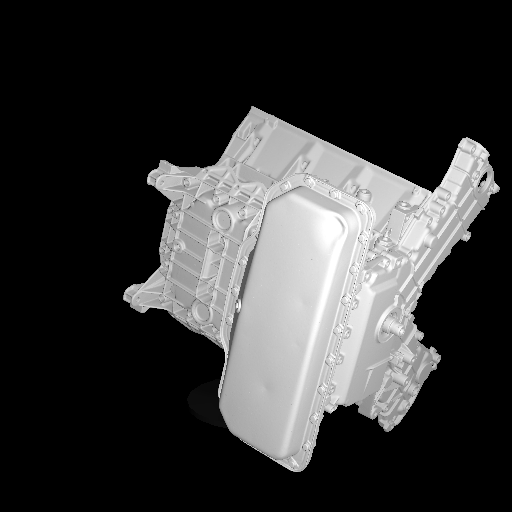
\includegraphics[width=\textwidth]{./Figures/right_exposure.png}
		\caption{Just Right}
	\end{subfigure}
	\begin{subfigure}[b]{0.32\linewidth}
		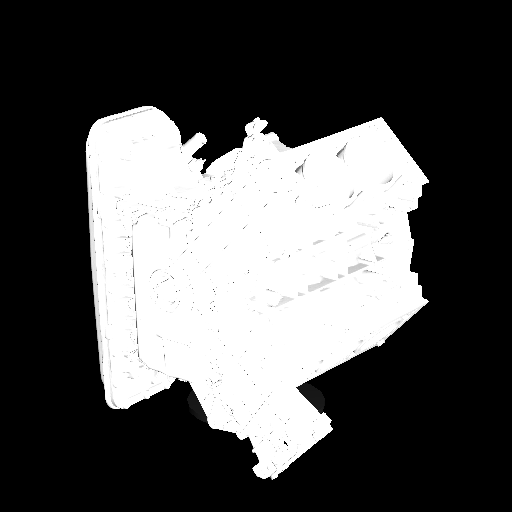
\includegraphics[width=\textwidth]{./Figures/wrong_exposure.png}
		\caption{Too much light}
	\end{subfigure}
	\decoRule
	\caption{Different exposure to the objects.}
	\label{fig:camera_exposure}
\end{figure}




\section{Data Preprocessing}
The raw data collected by Unity required further processing before it could be fed into the training models. 
\paragraph{Depth Map}
A depth map is a 1-channel image that contains information about the distance from the object surface to the camera center. It is stored as a 16-bit grayscale image, meaning that each pixel is in the range $\mathtt{0 - 65535}$. 

The raw depth maps in real data acquired by light scanners usually have missing pixels. To achieve a good match to the real data, a uniformly distributed noise was added to the synthetic data to randomly remove the valid pixels in the depth maps.
The simulated noise is uniformly distributed over the entire map with a certain noise intensity. A parameter $ \mu $ is used to control the intensity of the noise. It specifies the $ \mu $ pixel drop in percent. For example, at $ \mu-10 $, 10\% of the pixels are randomly removed. For each scene, the noise operation is based on a random $ \mu $ in a range $ \left[0, 50\right] $. In some scenes there are more missing pixels, in others less. The random noise intensity also allows the model to learn scenarios not only with noise, but also with low noise or even no noise.
Figure \ref{fig:noise-intensity} shows the noise effect at different $ \mu $.



%% add noise image
\begin{figure}[!h]
	\centering
	\captionsetup{width=\linewidth}
	{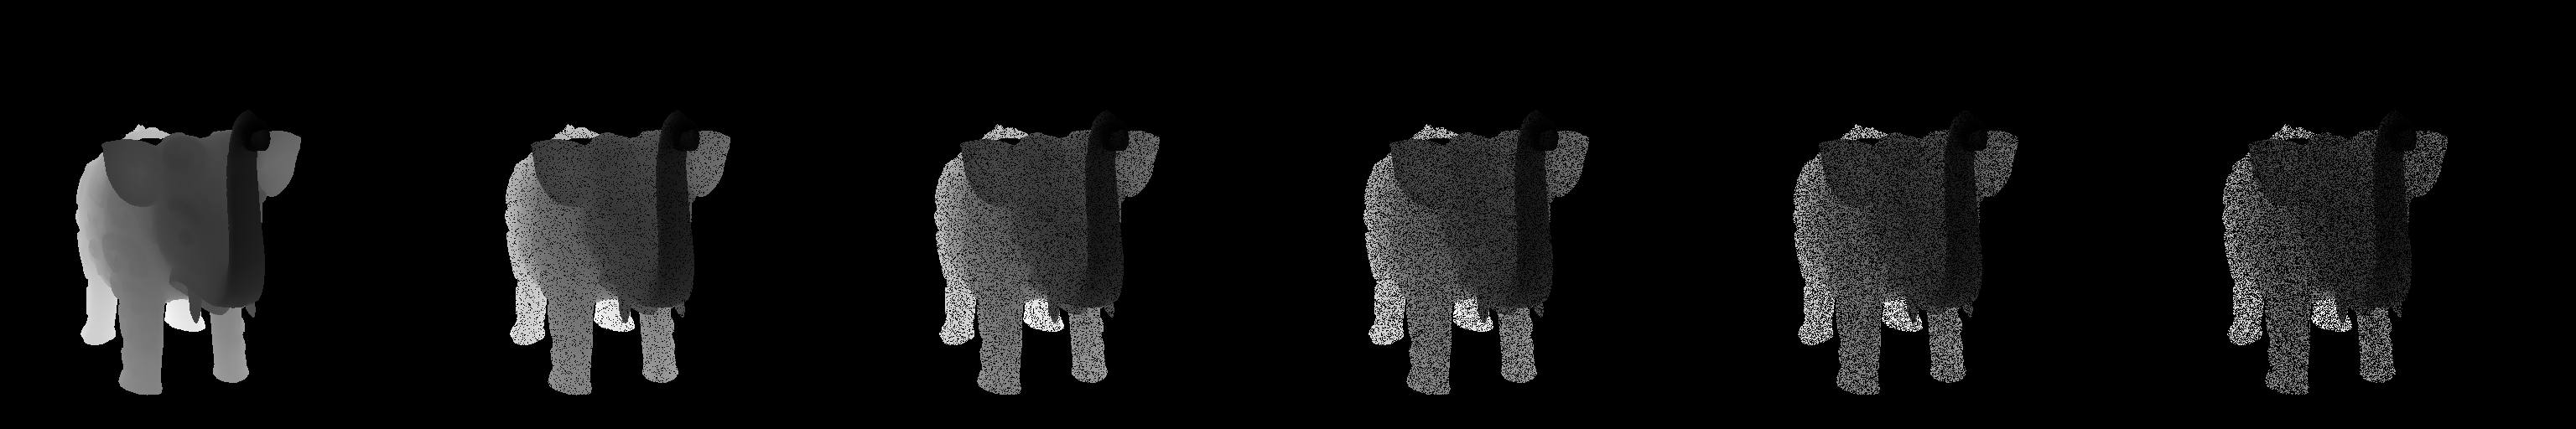
\includegraphics[width=\textwidth]{./Figures/add_noise_depth.png}}
	\decoRule
	\caption{From left to right: Noise-intensity on $ \mu-0$, $\mu-10$, $\mu-20$, $\mu-30$, $\mu-40$, $\mu-50$. Object Name: \textit{elephant-zun-lid}.}
	\label{fig:noise-intensity}
\end{figure}

%\begin{figure}[h!]
%	\centering
%	\begin{tikzpicture} 
%		% reference lines
%		\node[inner sep=10pt] (input) at (0,0)
%		{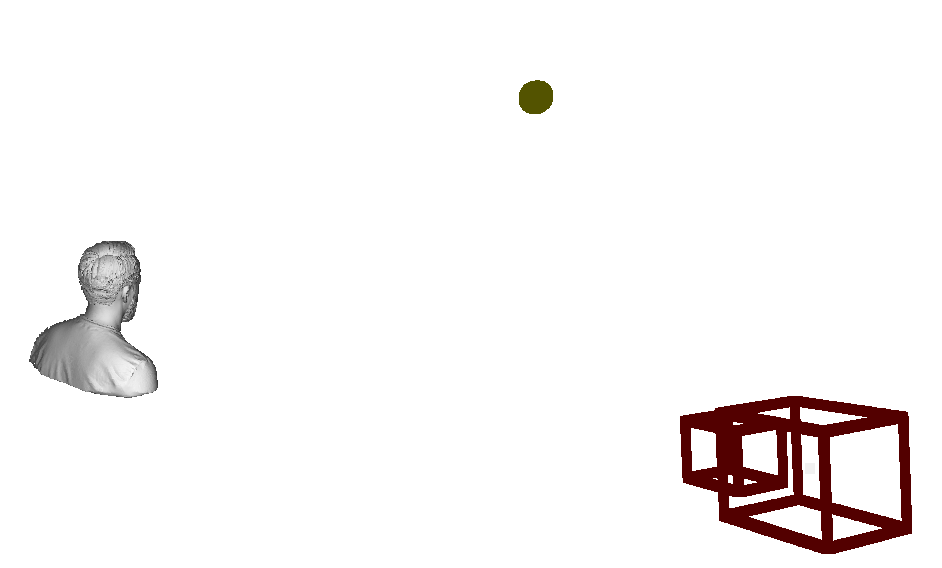
\includegraphics[width=\linewidth]{./Figures/ply_config.png}};
%		
%		%		\draw[thick,dashed]	(0,0) -- (10,0) ; % bottom
%		%		\draw[thick,dashed]	(0,3) -- (10,3) node[pos=0.9, above] {image plane}; % middle
%		%		\draw[thick,dashed]	(0,6) -- (10,6); % top
%		% camera 
%		%		\filldraw[black] (5,0) circle (2pt) node[anchor=south west]{Camera Position};
%		% world point 
%		%		\filldraw[black] (2,2) circle (2pt) node[anchor=north west]{Point};
%		% image point
%		%		\filldraw[black] (6,3) circle (2pt) node[anchor=north west]{Pixel};
%		% similiar triangles
%		%		\draw[thick] (0,0) -- (2,6); % AB
%		%		\draw[thick] (5,0) -- (7,6); % AC
%		%		\draw[thick] (5,6) -- (7,6) node[midway, below] {$ X $}; % BC
%		%		\draw[thick] (5,3) -- (6,3) node[midway, below] {$ u $};
%		%		% measure arrows
%		%		\draw[thick, <->] (4,0) -- (4,3) node[midway, left] {$ fk_u $};
%		%		\draw[thick, <->] (3,0) -- (3,6) node[pos=0.3, left] {$ Z $};
%	\end{tikzpicture}	
%	\caption{Data Collection configuration}
%	\label{fig:depth-triangulation}
%\end{figure}
The depth map is converted to a 3D vertex map after adding the noise.
Consider a 3-dimensional Euclidean space. The $ X $ and $ Y $ axes are perpendicular to each other align with the direction of width and height of the depth map separately. The $ Z $ axis is point inward (i.e., from view point to the depth map). The depth provided in the depth map is the distance from camera center to the object surface. Thus, in order to find the corresponding 3D vertex map $ \textbf{V}_C $ with respect to the camera coordinate system, we only need to multiple the depth matrix $ \textbf{Depth} $ with the point direction matrix $ \textbf{Dir} $.

\begin{dgroup*}
	\begin{dmath*}
		\textbf{V}_C = \textbf{Depth} \odot \textbf{Dir}
	\end{dmath*}
\end{dgroup*}

For the direction $ \textbf{Dir}(x,y,z) $ of a point $ \textbf{V}(x,y,z) $, it's X and Y components can be mapped from the corresponding pixel position $ (u,v) $ on the depth map, whereas the Z component is the focal length $ fk $ in pixels. Then we have to further normalize it to an unit vector.

\begin{dgroup*}
	
	\begin{dmath*}
		\textbf{Dir}(x, y, z) = \dfrac{(u, v, fk)}{\|(u, v, fk) \|^2_2}
	\end{dmath*}

\end{dgroup*}
Conversion of a point from the camera coordinate system to the world coordinate system using the extrinsic matrix $ R $ and $ t $
\[\textbf{V}_W = \textbf{V}_C R+t \]


%% How to represent input tensor, to make it fast converse
The sizes of the individual training objects are different. We normalized them to a unit scale so that they have a relatively similar distance from the camera.
In Figure \ref{fig:data_range} we have plotted the variations in value in each axis before normalization. Table \ref{tab:data_range} gives a quantitative evaluation of the corresponding average values. 

The normalization was performed as follows. First, the points are translated to the original point as much as possible, then the range value of an axis is chosen as the scaling factor, and the points are normalized to unit vectors. The equation is represented as follows

\begin{dgroup*}
	\begin{dmath*}
		X_n =\frac{X-\min(X)}{s}
	\end{dmath*}
	\begin{dmath*}
		Y_n = \frac{Y-\min(Y)}{s}
	\end{dmath*}
	
	\begin{dmath*}
		Z_n = \frac{Z-\min(Z)}{s}
	\end{dmath*}
	\begin{dmath*}
		s = \max(X)-\min(X)
	\end{dmath*}
\end{dgroup*}
where $ s $ is a scaling factor calculated as the range of the $ X $ axis, but theoretically it can also be the range of $ Y $ or $ Z $ axis.


\begin{figure}[!h]
	\centering
	\captionsetup{width=\linewidth}
	\begin{subfigure}[b]{0.49\linewidth}
		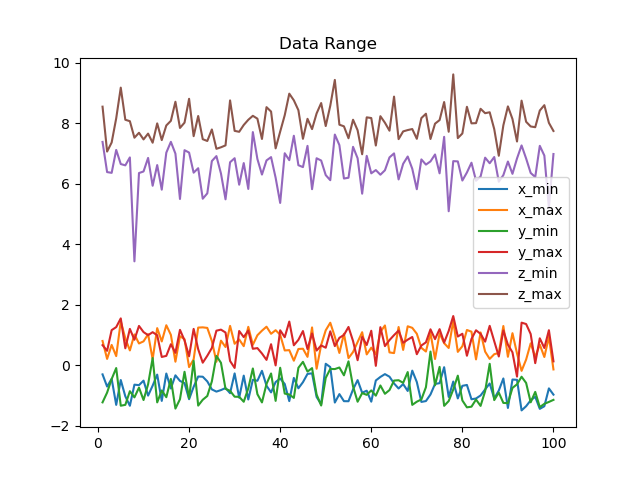
\includegraphics[width=\textwidth]{./Figures/Data_Extreme.png}
		\caption{Extreme Values in each axis }
	\end{subfigure}
	\begin{subfigure}[b]{0.49\linewidth}
		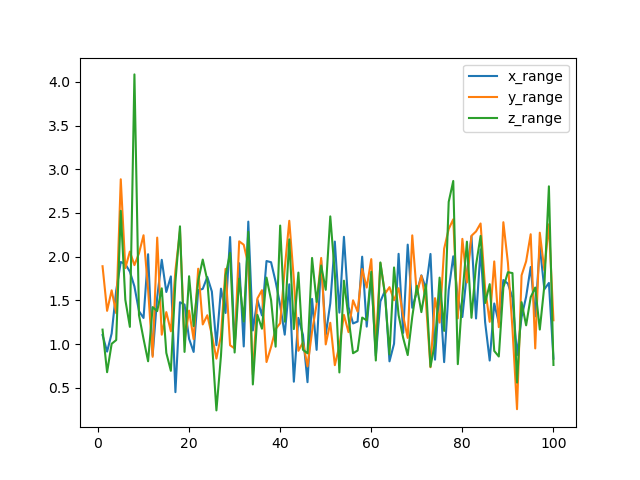
\includegraphics[width=\textwidth]{./Figures/Data_Range.png}
		\caption{Vertex Range in each axis}
	\end{subfigure}
	\decoRule
	\caption{The position fluctuation of the points in 100 Vertex Maps. 
		Left: Extreme values in 3 axes; Right: Vertex range in 3 axis.}
	\label{fig:data_range}
\end{figure}

\begin{table}[th]
	\centering
	\captionsetup{width=\linewidth}
	\begin{tabular}{c | c c c}
		\toprule
		\tabhead{Axis} & \tabhead{Scale} & \tabhead{Min} & \tabhead{Max}\\
		\midrule
		X & 1.48 & -0.75 & 0.73\\
		\hline 
		Y & 1.56 & -0.76 & 0.80\\
		\hline 
		Z & 1.47 & 6.53 & 8.00\\
		\bottomrule
	\end{tabular}
	\caption{ The fluctuation of extreme values and their ranges in 100 random training items. }
	\label{tab:data_range}
\end{table}




\paragraph{Image}

The grayscale image can be used for the photometric stereo method and also as readable information for humans. Since the image captured by the camera is in RGB format, we need to convert it to grayscale to fit our models. This is done using the following equation.
\[ gray: \frac{R+2G+B}{4}  \]

\paragraph{Normal Map}
The normal map is the tangential surface normal stored in an 8-bit/channel RGB image. The surface normal $ (n_x, n_y, n_z) $ and the corresponding RGB color $ (R,G,B) $ can be converted using the following equation:

\begin{dgroup*}
	\begin{dmath*}
		n_x = \frac{R}{255} \cdot 2 - 1
	\end{dmath*}
	\begin{dmath*}
		n_y = \frac{G}{255} \cdot 2 - 1
	\end{dmath*} 
	\begin{dmath*}
		n_z = 1-\frac{B}{255} \cdot 2
	\end{dmath*}
\end{dgroup*}

%In order to save training time, we compress the dataset in PyTorch format. The structure of a single item is shown in Table \ref{tab:tensor-structure}.
%\begin{table}[H]
%	\centering
%	\captionsetup{width=\linewidth}
%	\begin{tabular}{l | l}
%		\toprule
%		\tabhead{Name} & \tabhead{Content} \\
%		\midrule
%		\multirow{3}{*}{input-tensor}  & Vertex \\  & Image \\  & Light Direction \\
%		\hline
%		\multirow{3}{*}{output-tensor}  & GT-Normal \\ & Image \\ & GT-Light-Direction \\
%		\hline
%		Light position & light position \\
%		\hline 
%		Camera Matrix  & K,R,t\\
%		\hline 
%		Depth Range  & minDepth, maxDepth\\
%		\bottomrule
%	\end{tabular}
%	\caption{The structure of a single tensor in the dataset.}
%	\label{tab:tensor-structure}
%\end{table}
